\section{Additional}
\subsection{Speeding up Aging}

\begin{frame}[c]{Werner Syndrome}
    \large
    \begin{itemize}[<+(1)->]
        \item 'Premature aging', median age of death: 47
        \item Autosomal Recessive (does not affect carrier)
        \item Caused by mutation in WRN gene
        \item WRN important for DNA-Repair, especially after oxidative damage \cite{szekely2005werner}
    \end{itemize}

\end{frame}


\begin{frame}[c]{Artifially speed up aging}
    \large
    Study with mice injected restriction enzyme activate with drug to induce
    repeated DNA damage, they age considerably faster. Same with knocking out SIRT1 and others
\end{frame}

\section{Common Pathways}

\subsection{Effects of harsh conditions}

\begin{frame}[c]{Life Expectancy after Cancer}
    \large
    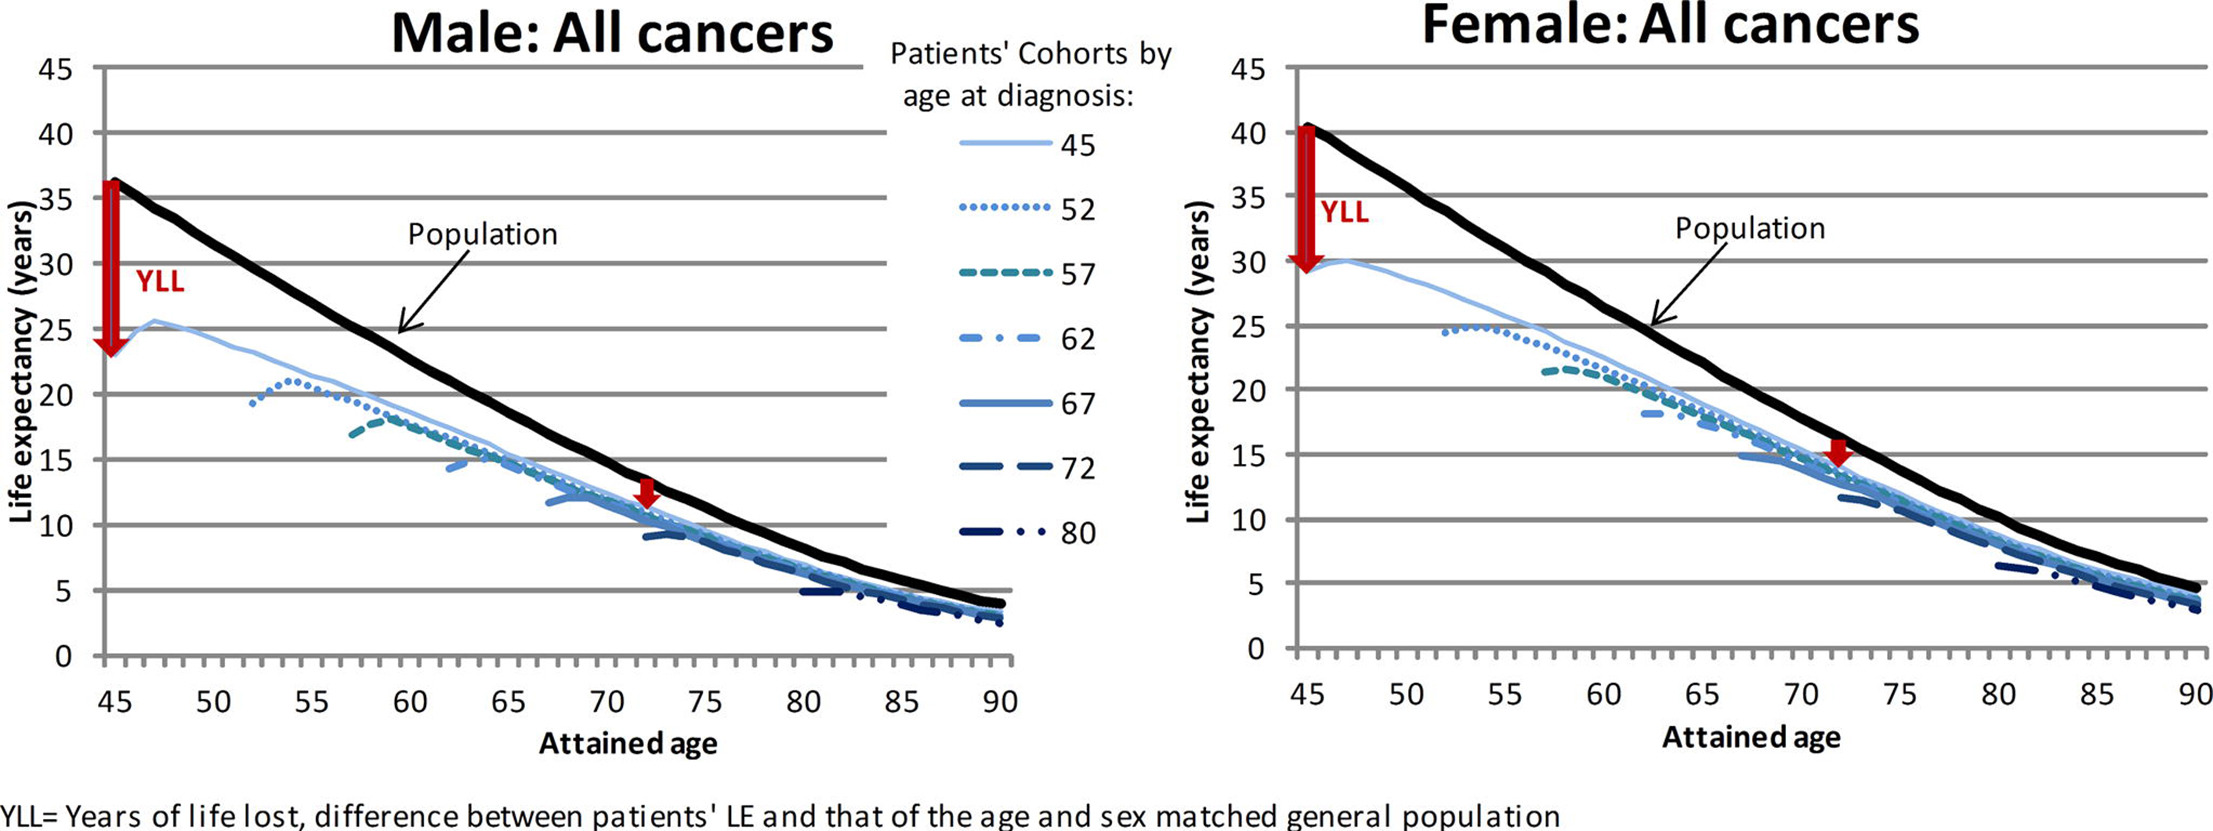
\includegraphics[width=\textwidth]{all_cancers_LE} \\
    \cite{botta2019changes}
    \newline
    \newline
    \pause
    Conclusion: Cancer causes the underlying \\ 'aging clock' to speed up \\
    reformulate to indication or something
\end{frame}

\begin{frame}[c]{Life Expectancy with Diabetes}
    \large
    Life Expectancy is at least 10 years lower with Diabetes Type 1
    \cite{livingstone2015estimated} and at least 5 years lower with Diabetes Type
    2 \cite{untitled1:online}.
    \newline
    \newline
    \pause
    Conclusion: Diabetes causes the underlying \\ 'aging clock' to speed up
\end{frame}


\begin{frame}[c]{Life Expectancy under Physiological Stress}
    \large
    \begin{aquote}{John S Wentworth \cite{Homeosta76:online}}
    There's a qualitative general pattern that various kinds of physiological
        stress - exposure to radiation or harsh chemicals (including smoking),
        chronic infection, malnutrition, sleep deprivation, etc - tend to
        accelerate aging.
    \end{aquote}
    find papers showing that these things cause hallmarks of aging to deteriorate
\end{frame}


\subsection{Diseases of Aging}

\begin{frame}[c]{Similarities of Diseases of Aging}
    \large
    \cite{CorePath13:online}
    At the cellular level:
    \begin{itemize}[<+(1)->]
        \item Decrease in cell count
        \item Increase in damaged proteins/DNA/fats
        \item Inflammation
    \end{itemize}
    \pause

    Roughly this pattern for:
    \begin{multicols}{2}
    \begin{itemize}[<+(1)->]
        \item Alzheimers
        \item Arthritis
        \item Atherosclerosis
        \item Muscle loss
        \item Osteoporosis
        \item Many more
    \end{itemize}
    \end{multicols}
\end{frame}

\begin{frame}[c]{Existence proof for common pathways}
    \large
    \begin{aquote}{John S Wentworth}
        someone who has one severe illness early is likely to have others
    \end{aquote}

    \pause
    Most severe illnesses cause the 'aging clock' to speed up. Most diseases of
    aging have similar characteristics. This is direct evidence that there are
    {\em few underlying root causes} for aging.
\end{frame}


\section{Hallmarks of Aging}

% \begin{frame}[c]{Overview of Core Mechanisms}
%     \large
%     \begin{itemize}[<+(1)->]
%         \item DNA Damage
%         \item Loss of Epigenetic Information
%         \item Mitochondria low-energy state
%         \item Telomere attrition
%         \item Unsuppressed Transposons
%     \end{itemize}
% \end{frame}


\subsection{DNA Damage}
\begin{frame}[c]{DNA Damage}
    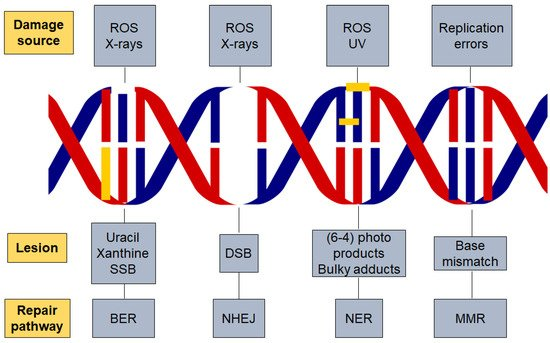
\includegraphics[width=\textwidth]{dna_damage} \\
    \cite{alhmoud2020dna}
    % turnaround a few days at most, does not accumulate - but, increase causes aging, just isn't root cause
    \pnote{Base excision repair (BER), nucleotide excision repair (NER), non-homologous end joining (NHEJ), reactive oxygen species (ROS) and DNA mismatch repair (MMR)}
\end{frame}

\subsection{Epigenetic information Loss}
\begin{frame}[c]{Epigenetic Information Loss}
    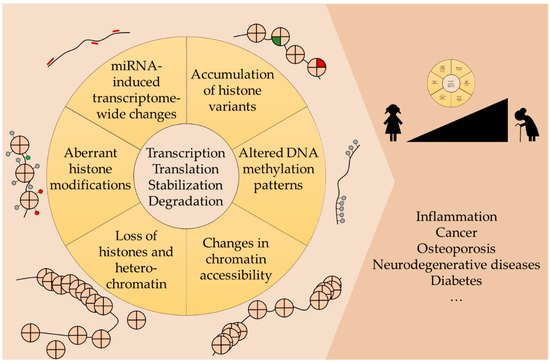
\includegraphics[width=\textwidth]{epigenetics_aging} \\
    \cite{saul2021epigenetics} \\
    % The state of an organisms epigenetics are a strong predictor for time to death \cite{lu2019dna} \\
\end{frame}

\subsection{Damaged Mitochondria}
\begin{frame}[c]{Mitochondria}
    Produce energy, explain fail-state and ROS
\end{frame}

\subsection{Telomeres}
\begin{frame}[c]{Telomeres}
    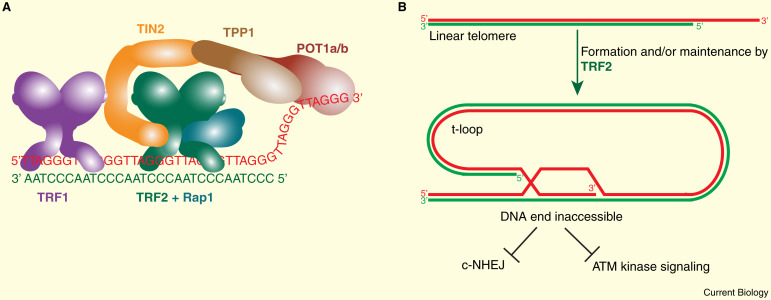
\includegraphics[width=\textwidth]{telomere_caps} \\
    \cite{schmutz2016shelterin} \\
\end{frame}

\begin{frame}[c]{Telomere attrition}
    \large
    \begin{itemize}[<+(1)->]
        \item Telomere length is only really relevant for stem cells, others don't divide
        \item Telomerase is active in stem cells
        \item True telomere damage cannot be repaired, so telomeres accumulate damage \cite{NintilTh68:online}
        \item Short telomeres cause cells to induce apoptosis
        \item So it's a good measure for total cell damage \cite{victorelli2017telomeres} 
    \end{itemize}
\end{frame}

\subsection{Transposons}
\begin{frame}[c]{Transposons}
    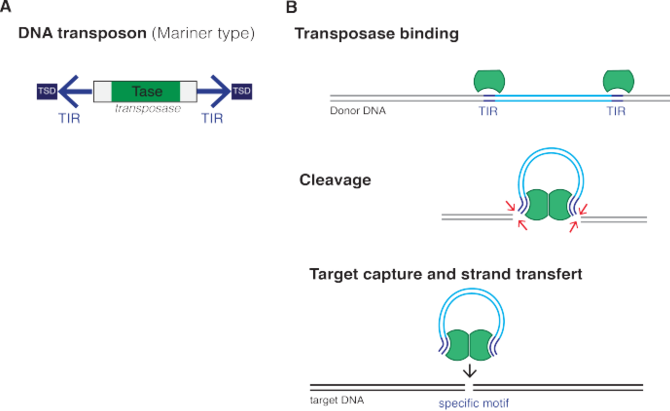
\includegraphics[height=0.8\textheight]{transposon} \\
    \pnote{
    explain transposons quick \\
    cause DNA damage, though rather additionally, as species without transposons also age \\
    about 50\% of human dna are 'dead' (broken) transposons, about 100 (of 11 major families) are still active \\
    they are suppressed most of the time, but 'let loose' a bit on other pressing matters (e.g. repairing dna damage) \\
    try to find good pictures \\
    mention that studies are being conducted currently \\
    }
    \cite{walter2015transposon} \\
    Also: mice from older fathers live shorter \cite{xie2018epigenetic}
\end{frame}

\subsection{Timeframes}

\begin{frame}[c]{Timeframes for Pathways}
    \large
    \begin{itemize}[<+(1)->]
        \item DNA Damage: Repaired within Hours or faster \cite{frankenberg1989review}
        \item Senescent Cells: Removed within Days \cite{karin2018senescent}
        \item Epigenetic Markers: Varies, but most are replaced within Weeks \cite{ginno2020genome} \cite{yamagata2012rapid}
    \end{itemize}
    \pause
    Conclusion: Either the amount of Damage/Senescent Cells increases or Reparation/Removal decreases
\end{frame}

\section{Root Causes}
\subsection{Assumed Root Causes}

\begin{frame}[c]{Problem: Many Theories}
    \large
    \begin{itemize}[<+(1)->]
        \item Everything is interlinked
        \item Very hard to distinguish cause and effect
        \item At least one Theory for every Hallmark
        \item Every prestigious lab has its own Theory
        \item A lot of speculation on all sides
        \item Unclear if we can already see the full picture
        \item More research is needed
    \end{itemize}
\end{frame}

\addtocounter{framenumber}{1}
\begin{frame}[standout]
    Disclaimer: Purely Speculation including many Unknowns
\end{frame}

\begin{frame}[c]{Mitochondrial dysfunction}
    \large
    Turns out, mitochondrial dysfunction accounts for telomere-dependent senescence \cite{passos2007mitochondrial}.
\end{frame}


\begin{frame}[c]
    \large
    Assumed root causes: free radicals and transposon damage \\
    Maybe not in too much detail? Could fill 30min itself \cite{CorePath13:online} \\
    \pause

    p21 and reactive oxygen feedback for senescence \cite{passos2010feedback}
\end{frame}



\subsection{Open Questions}

\begin{frame}[c]{Questions Unanswered}
    \begin{itemize}[<+(1)->]
        \item Where are the ROS produced? Mitochondria are the top candidate - there’s a known mechanism for ROS production by mitochondria, as well as experimental evidence that mitochondrion-targeted antioxidants specifically reduce ROS-induced damage.
        \item How do the ROS and/or damaged molecules move between compartments, e.g. nucleus/cytoplasm/extracellular? I have seen very little on this, and consider it a major blindspot. I’m not sure if it’s a blindspot for the field or if I just haven’t found the right cluster of papers.
        \item Are the quantitative changes in DNA/protein/fat damage compatible with a single underlying cause? Do they match plausible estimates of ROS from dysfunctional mitochondria? Again, I haven’t seen Fermi estimates here, but I’d like to.
        \item Why is the immune system degradation related? It does degrade similarly over time, does it 'age' as well? This implies at least a second independent pathway and approach
    \end{itemize}
\end{frame}



\section{Slowing down Aging (additional)}

\subsection{Parabiosis}

\begin{frame}[c]{Parabiosis (Blood Exchange)}
    \scriptsize
    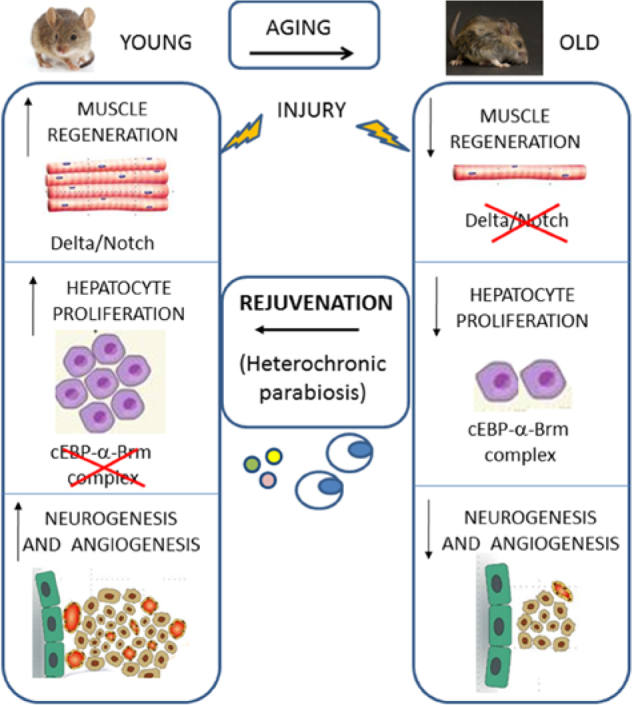
\includegraphics[height=0.9\textheight]{parabiosis_effects} \\
    Source: \cite{conese2017fountain}
    \pnote{
        Connecting blood circulation of old and young \\
        Benefits to old, donwsides to young mice \\
        Can be brought to biological equilibrium
        \par
        Works by Hormones, Immune defenses and \\
        other Growth Factors/regulation in the blood \\
        as well as nutrients and stem cells
        \par
        hepatocyte = important liver cell \\
        angiogenesis = forming new blood vessels
        \par
        Next: How good is it? (Evaluation)
    }
\end{frame}

\begin{frame}[c]{Method Evaluation: Parabiosis}
    \large
    % Parabiosis (heterochronic parabiosis) is putting young blood into old mice, to make the old mice biologically younger. This is achieved in the lab by connecting the circulatory systems of young mice and old mice. Certain factors in the blood help to rejuvenate muscle, heart brain and liver tissues in old mice and restore their biological function.

% Equivalent procedures that modify the compounds within blood in humans such as apheresis (blood filtering) could be used to slow aging in humans and thereby prevent or slow the progression of many types of age-related diseases including Alzheimer's disease.

% Recently, a group of Russian biohackers recently took part in the first plasma dilution experiments in humans. In a research context, the safety and effectiveness of apheresis is being tested in a clinical trial in humans by the company Alkahest.

    \textbf{Hallmarks affected}:
    \begin{aquote}{\cite{conese2017fountain}}
        In principle, the heterochonic parabiosis reverts all phenotypic and molecular hallmarks of ageing by transferring soluble factors and cells.
    \end{aquote}
    % \begin{itemize}[<+(1)->]
    %     \item Stem cell exhaustion
    %     \item Cellular senescence
    %     \item Altered intercellular communication
    % \end{itemize}
    % parabiosis reverses age-related decline by targeting several hallmarks of aging including stem cell exhaustion, cellular senescence and altered intercellular communication (inflammation).

    \pause
    Alternatives: Blood Filtering and (Growth) Hormone Therapy. \\
    \pause
    \textbf{Status: In clinical trial}, e.g. \cite{AStudyto73:online}.
    \pnote{
        soluble = 'Löslich' \\
        also transfers bone marrow (stem cells) \\
        Source: \cite{lukic2005shared} \\
        \par
        Alternatives, because downsides for young \\
        mice not neglegible
    }
\end{frame}

\subsection{Dietary Restriction}

\begin{frame}[c]{Dietary Restriction Pathways in Yeast}
    \scriptsize
    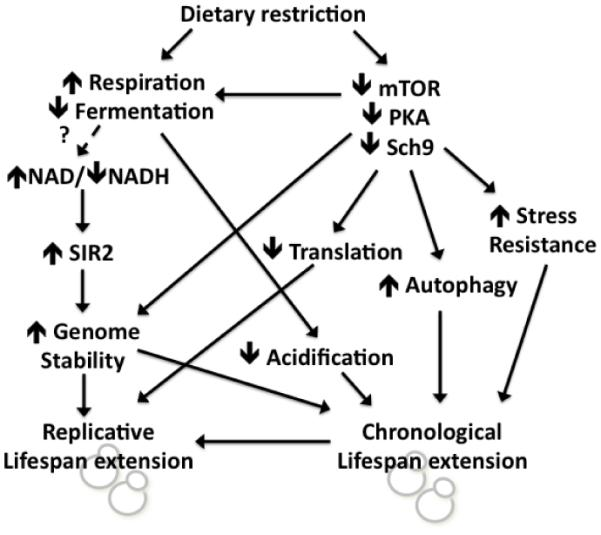
\includegraphics[height=0.85\textheight]{dietary_restrict_yeast} \\
    Source: \cite{kapahi2017dietary}
    \pnote{
        Fruit fly much more confusing, but similar
        \par
        Downregulation of mTOR receptors \\
        (mechanistic Target of Rapamycin)
        \par
        SIR -> increased dna damage repair \\
        Autophagy -> usually 10-20\% non-func protein \\
        'Starvation Mode': Be more efficient \\
        (also downregulate immune system)
        \par
        Next: Dietary Restriction Effects
    }
    % remove slide
\end{frame}

\begin{frame}[c]{Same Effects without Diet}
    \large
    Nutrient-Sensing pathways affected by Dietary Restriction, and easy to target:
    \begin{itemize}[<+(1)->]
        \item AMPK
        \item mTOR
        \item IGF-1
    \end{itemize}

    \pause
    Medications \textbf{in trial} to affect these pathways:
    \begin{itemize}[<+(1)->]
        \item Metformin \cite{TAMETarg47:online}
        % \item Metformin \cite{martin2013metformin}, \cite{TAMETarg47:online}
        \item Rapamycin \cite{Particip66:online}
        \item Many more ...
    \end{itemize}
    \pnote{
        AMPK = 5' AMP-activated protein kinase \\
        AMP = Adenosine Monophosphate = ATP -2P \\
        IGF-1 = Insulin-like-Growth-Factor 1 \\
        \par
        Large-scale studies to achieve same benefits \\
        without actual dietary restriction \\
        \par
        So how does it fare? How do they do? \\
        Next: Evaluation
    }
\end{frame}



\subsection{Cellular Reprogramming}

\begin{frame}[c]{(Epigenetic) Cellular Reprogramming: What is it?}
    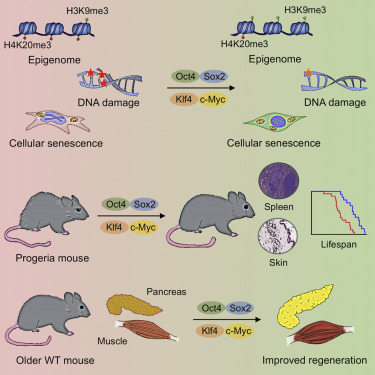
\includegraphics[height=0.85\textheight]{repr_overview} \\
    Source: \cite{ocampo2016vivo}
    \pnote{
        The idea is to 'reprogram' old cells \\
        to be like young cells
        \par
        Largely dependent on epigenome: dna markers \\
        Goal: Basically to reprogram the epigenome
        \par
        Next: Epigenetics
    }
\end{frame}


\begin{frame}[c]{Epigenetics: What is it?}
    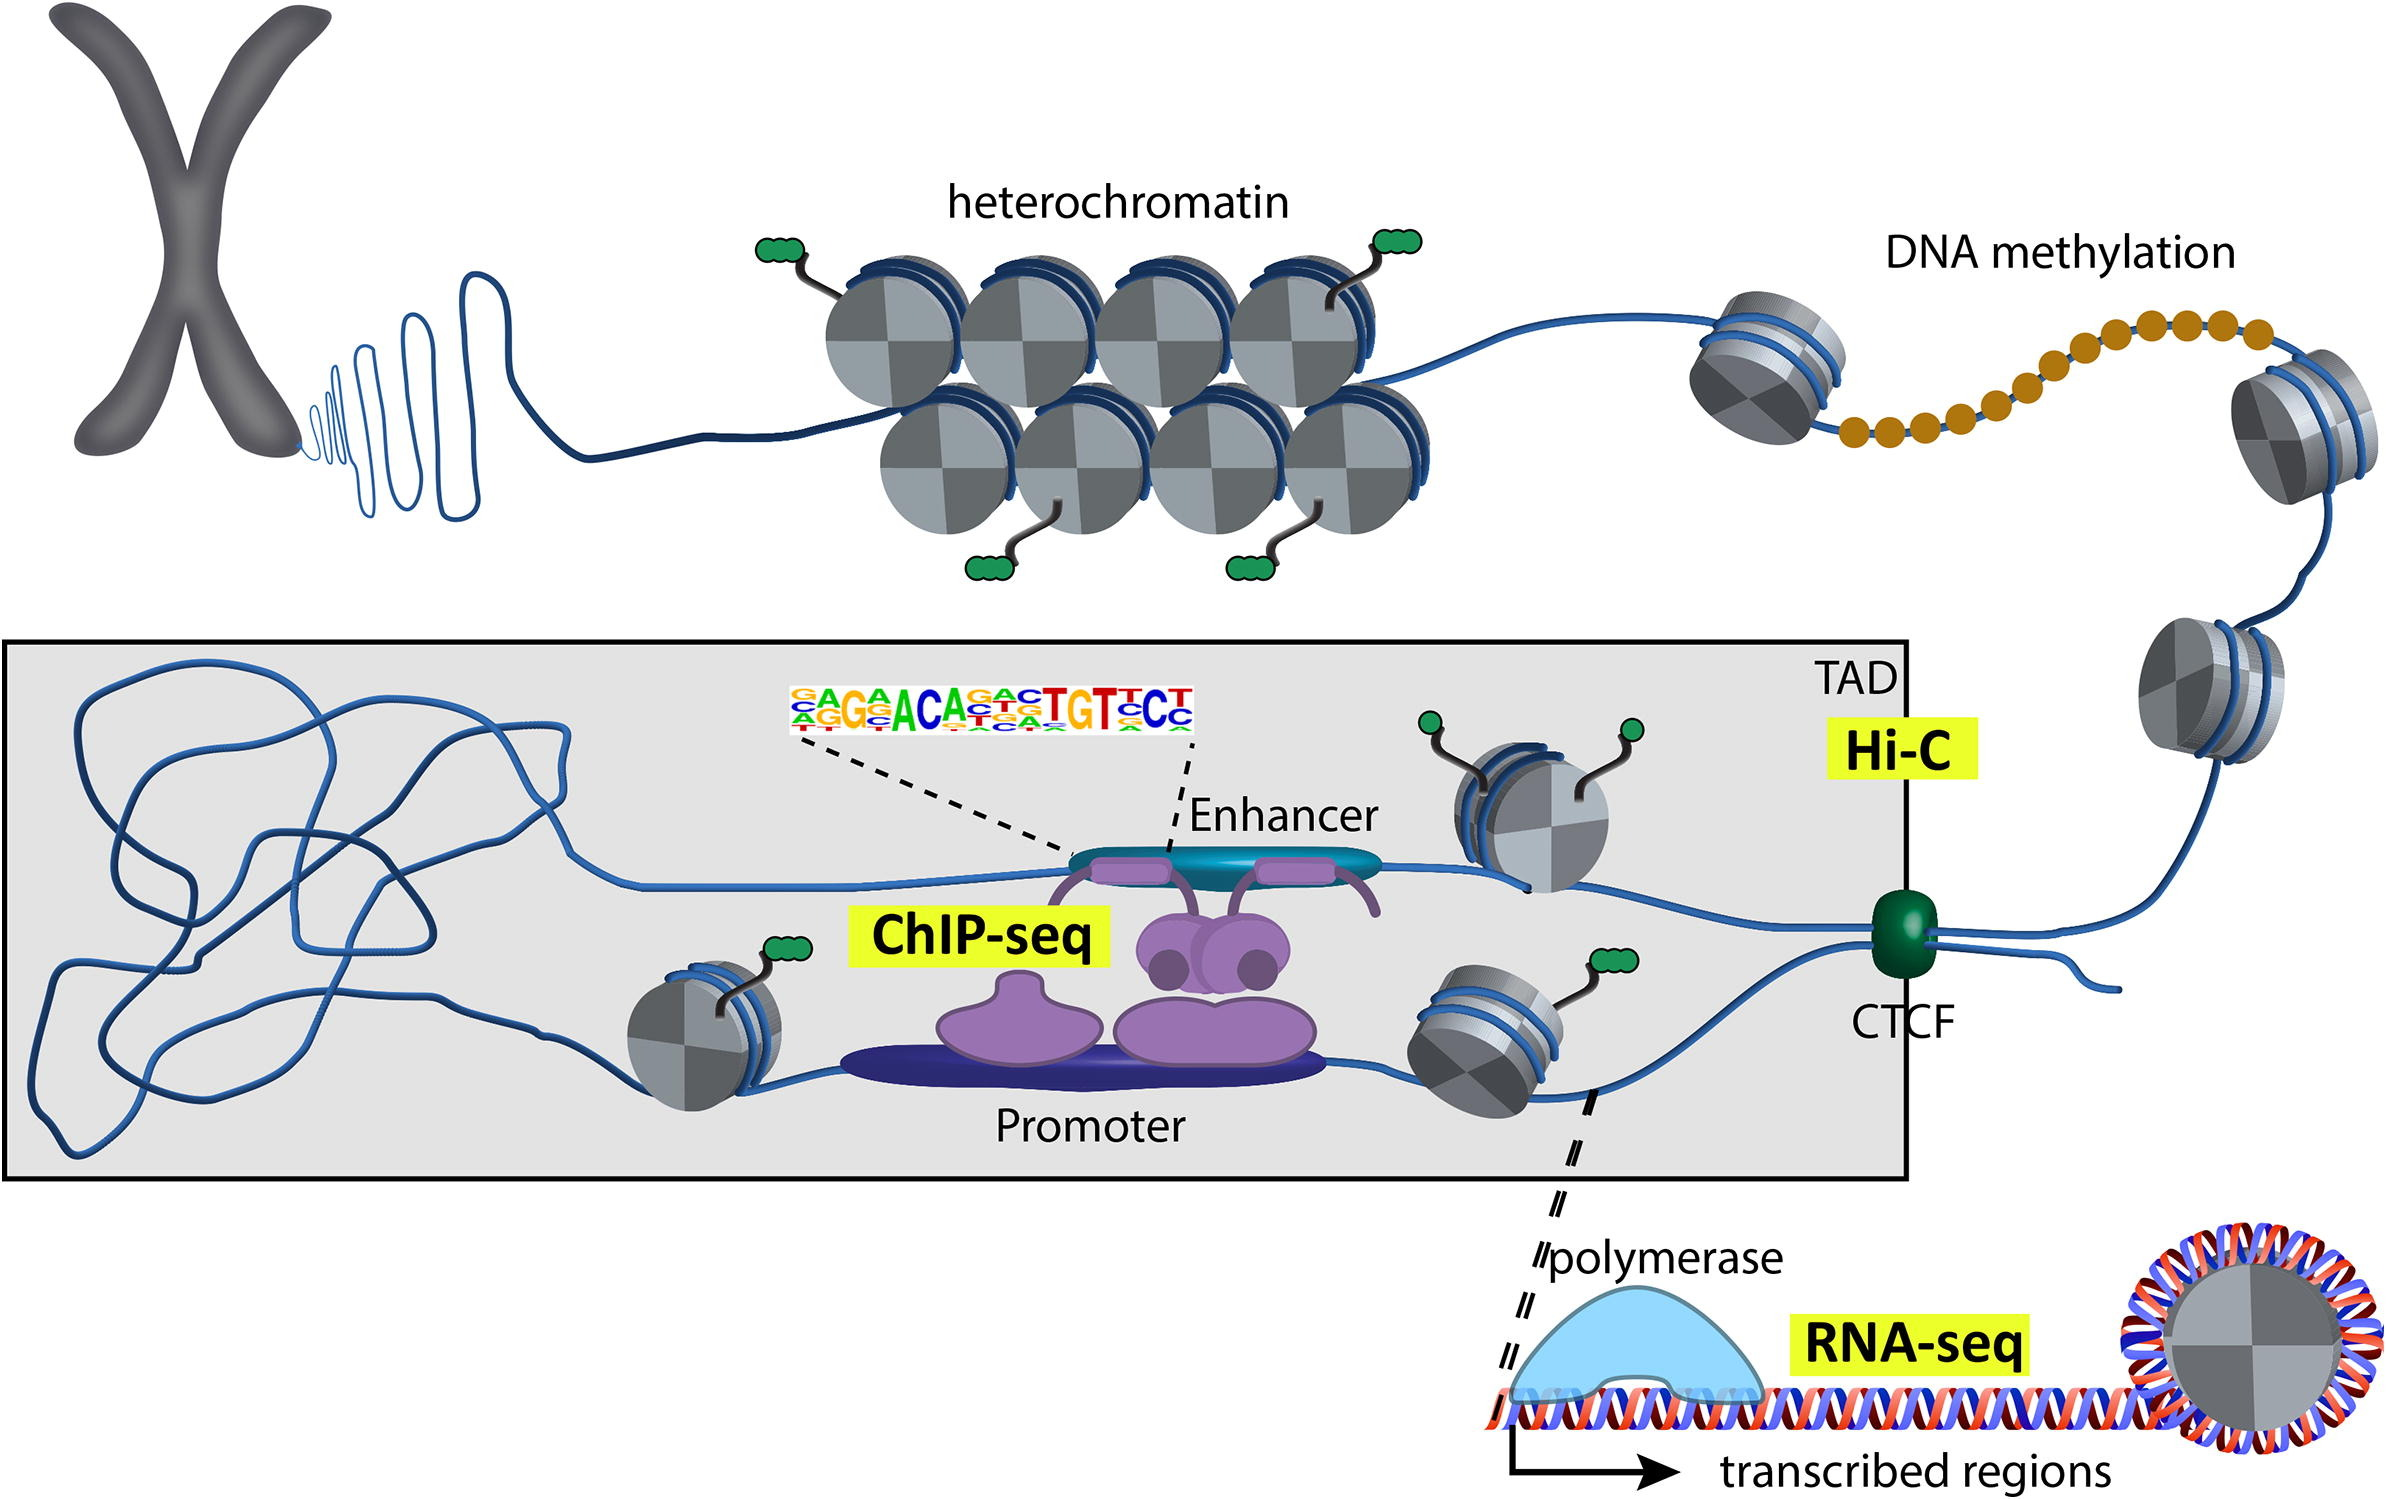
\includegraphics[height=0.85\textheight]{epigenetics} \\
    Source: \cite{hollbacher2020seq}
    \pnote{
        Epigenetics: many state machines as to \\
        what the cell is supposed to be doing \\
        by methylation certain parts of the genome \\
        can be modulated by messages/hormones
        \par
        decides which genes are being expressed/suppressed \\
        Can be thought of as 'cell identity' \\
        differentiation between muscle cell and skin cell
        \par
        'highest-level' regulation of what happens \\
        Danger lies in 'forgetting' own states \\
        Next: Cellular Reprogramming
    }
\end{frame}

\begin{frame}[c]{(Epigenetic) Cellular Reprogramming: What is it?}
    \large
    \begin{itemize}[<+(1)->]
        \item Basically: reset the corroding Epigenetic state to a 'younger' and functional one
        \item In fact, we can create induced pluripotent stem cells (iPSC) \cite{takahashi2006induction}
        \item Cells activated with Yamanaka-factors are indistinguishable (regarding aging-hallmarks) from younger versions of themselves
        \item Idea: only activate them long enough to reverse aging hallmarks, but keep cell identity
        \item Seems to complement well with senolytics \cite{ofenbauer2019strategies}
    \end{itemize}
    \pnote{
        When things start to go wrong, \\
        reset to a 'known working state'
        \par
        Originally, iPSC lost their cell identity \\
        iPSC more powerful and rare than stem cells
        \par
        Incredible potential for other treatments
        \par
        Next: Evaluation
    }
\end{frame}


\begin{frame}[c]{Method Evaluation: Cellular Reprogramming}
    \large
    \textbf{Hallmarks affected}: \\
    \begin{itemize}[<+(1)->]
        \item Mitochondrial Dysfunction
        \item Shortening of Telomere length
        \item Changes in Epigenetic markers
        \item Genomic Instability
        \item Cellular Senescence
    \end{itemize}
    \pause
    Lifespan extension: maximum by 20\% and median by 33\% \cite{ocampo2016vivo} \\
    \pause
    \textbf{State: in clinical trial}
    \pnote{
        mitochondrial function regulated by epigenetics \\
        energy-fail-states exist and hard to get out of \\
        stem cells have active telomerase \\
        close-to-senescent stem cells might exist, ask
        \par
        Next: Other Approaches
    }
\end{frame}

\subsection{Senolytics}

\begin{frame}[c]{Senolytics: Uses and Effects}
    \scriptsize
    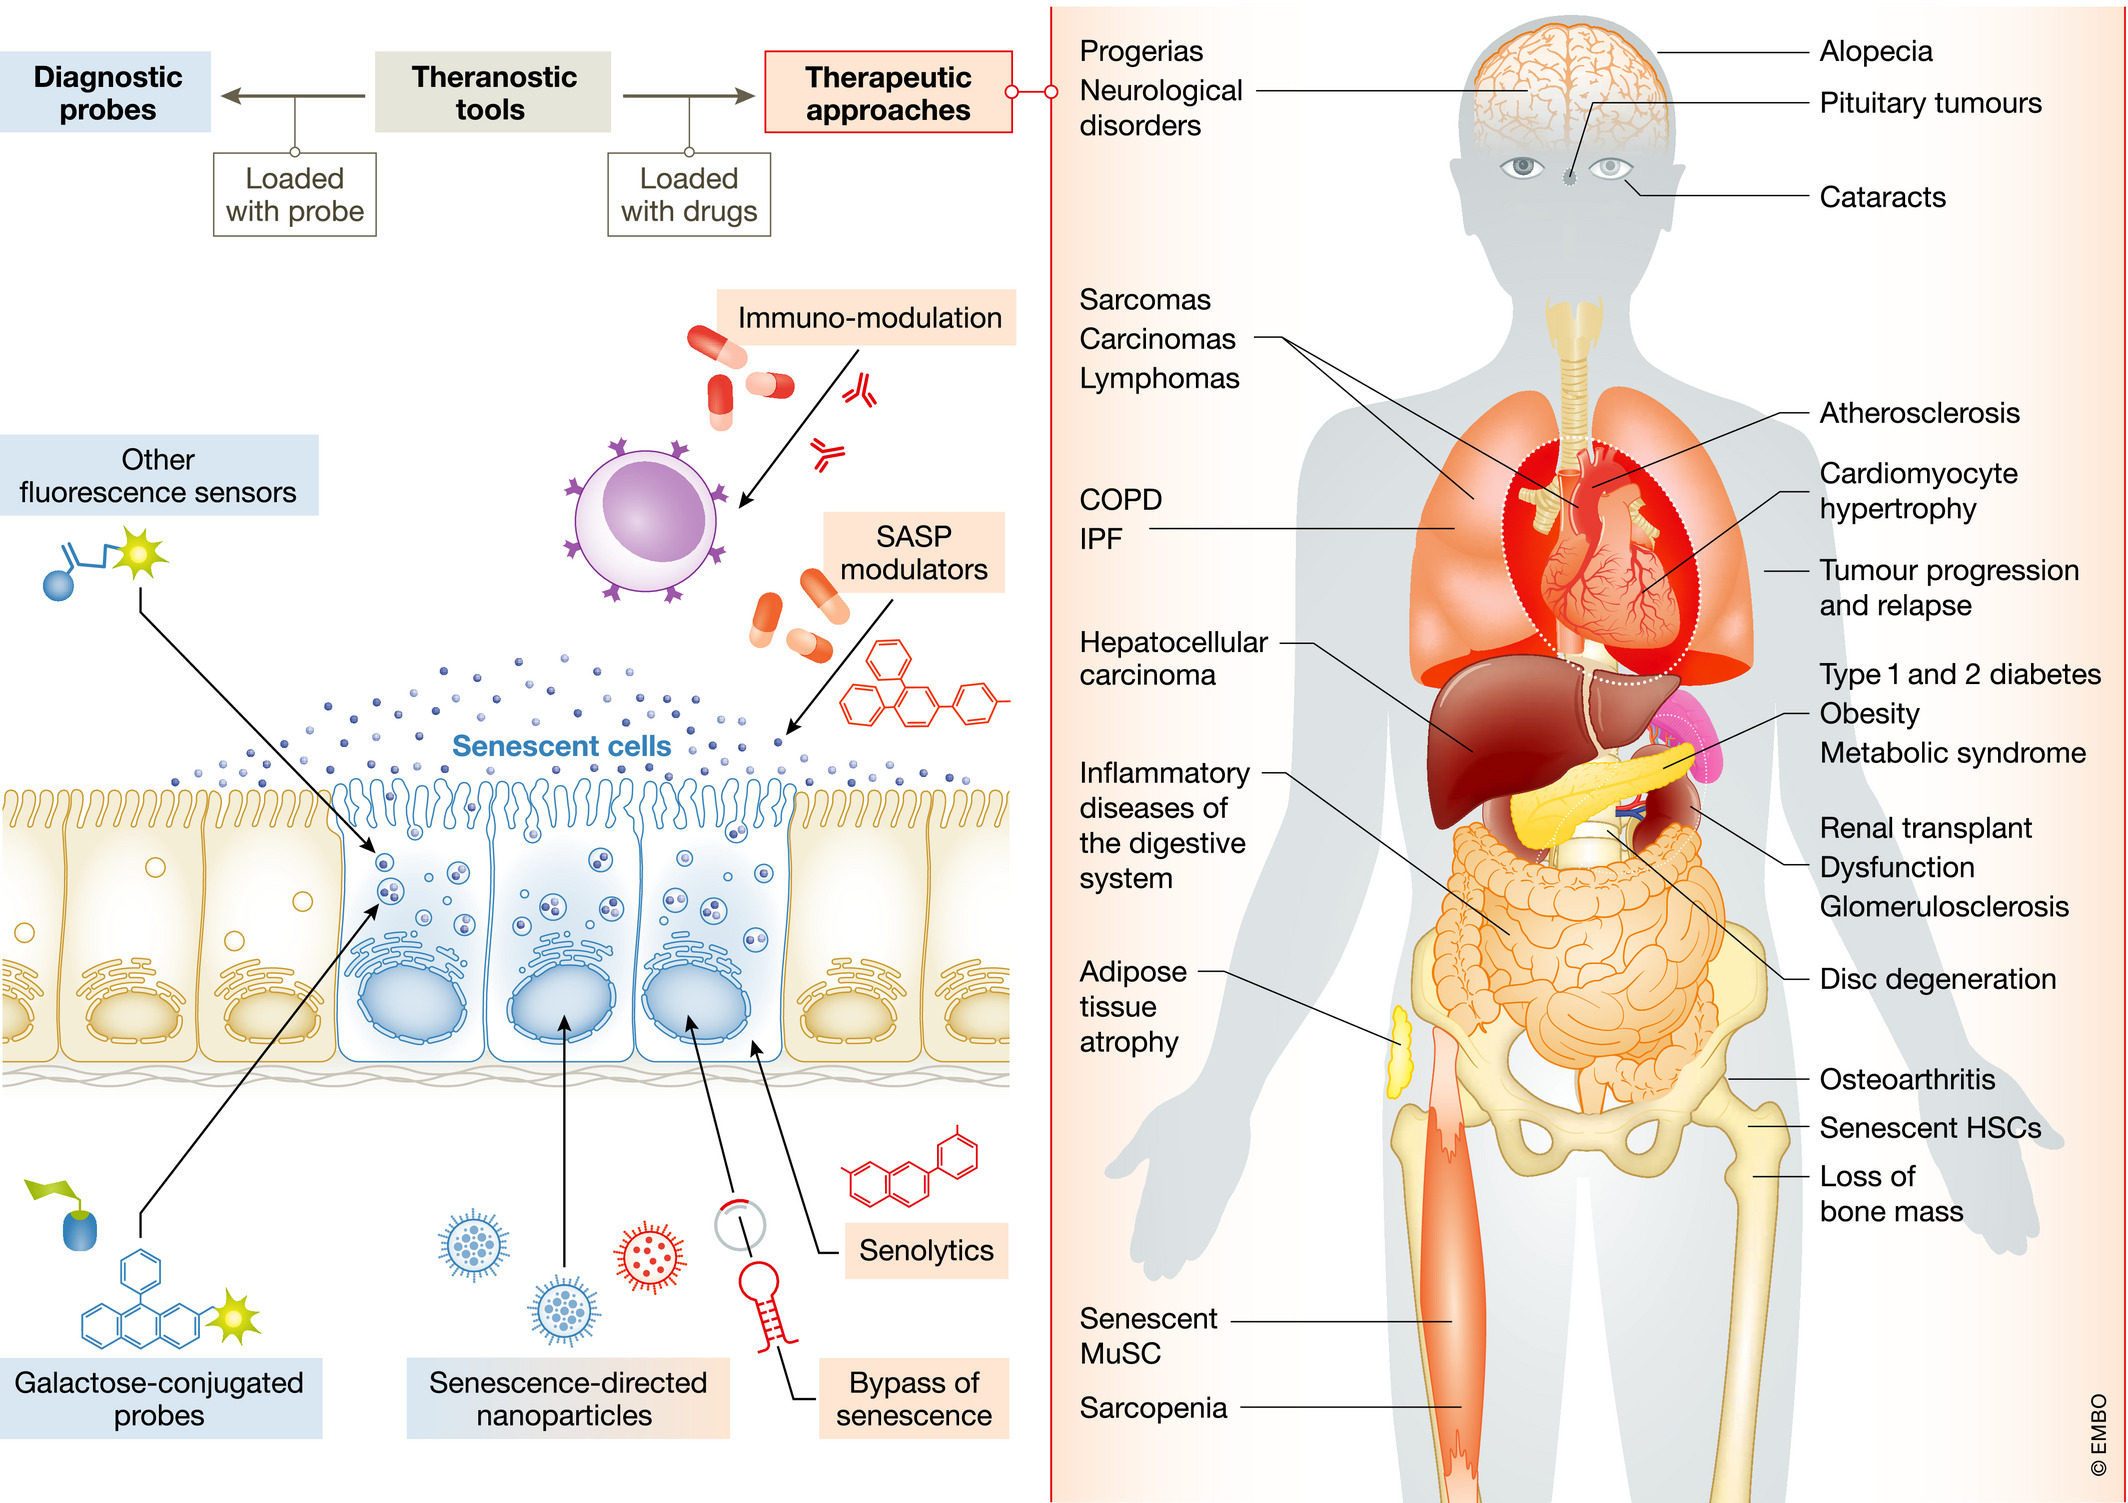
\includegraphics[height=0.85\textheight]{senescent_strategies} \\
    Source: \cite{paez2019targeting}
    \pnote{
        Right: Inflammation Diseases, usually when old \\
        Left: \\
        - e.g. Probes to detect senescence \\
        - Senolytics: inhibit pro-survival pathways \\
        -   Increasing apoptosis and immuno-clearance \\
        - SASP modulation: inhibit negative effects \\
        - Immuno-": Promote immune system clearance
        \par
        Next: Evaluation
    }
\end{frame}



\section{Misc}

\subsection{Problematic: Many Unknowns}

\begin{frame}[c]{Problem: Many Theories of Aging}
    \large
    \begin{itemize}[<+(1)->]
        \item Everything is interlinked
        \item Very hard to distinguish cause and effect
        \item At least one Theory for every Hallmark
        \item Every prestigious lab has its own Theory
        \item A lot of speculation on most sides
        \item Unclear if we can already see the full picture
        \item More research is needed
    \end{itemize}
    \pnote{Unclear if we have all the puzzle pieces \\ to solve it}
\end{frame}

\addtocounter{framenumber}{1}
\begin{frame}[standout]
    Disclaimer: Any misrepresentation or mistaken interpretation is due to my shortcomings
\end{frame}
